\section{LVars by example}\label{s:lvars-examples}

\emph{IVars} \cite{IStructures, id, CnC, monad-par} are a well-known
mechanism for deterministic parallel programming.  An IVar is a
\emph{single-assignment} variable \cite{Tesler-1968} with a blocking
read semantics: an attempt to read an empty IVar will block until the
IVar has been filled with a value.  LVars are a generalization of
IVars: unlike IVars, which can only be written to once, LVars allow
multiple writes, so long as those writes are monotonically increasing
with respect to an application-specific lattice of states.

Consider a program (written in a hypothetical language) in which two
parallel computations write to an LVar $\mathit{lv}$, with one thread
writing the value $2$ and the other writing $3$:
\begin{equation}
\begin{split}
& \LETPAR ~\_ = \putexp{\mathit{lv}}{3} \\
&  \letparspace ~\_ = \putexp{\mathit{lv}}{2} \\
&  \letspace \IN~ \GET~\mathit{lv}
\end{split}
\label{e:lvar-example-1}
\end{equation}
Here, @put@ and @get@ are operations that write and read LVars,
respectively, and the expression
\begin{displaymath}
\letparexp{x_1}{e_1}{x_2}{e_2;~\dots}{\mathit{body}}
\end{displaymath}
has \emph{fork-join} semantics: it launches concurrent subcomputations
$e_1, e_2, \dots$ whose executions arbitrarily interleave, but must
all complete before $\mathit{body}$ runs.  The @put@ operation is
defined in terms of the application-specific lattice of LVar states:
it updates the LVar to the \emph{least upper bound} of its current
state and the new state being written.

\begin{figure}
\centering
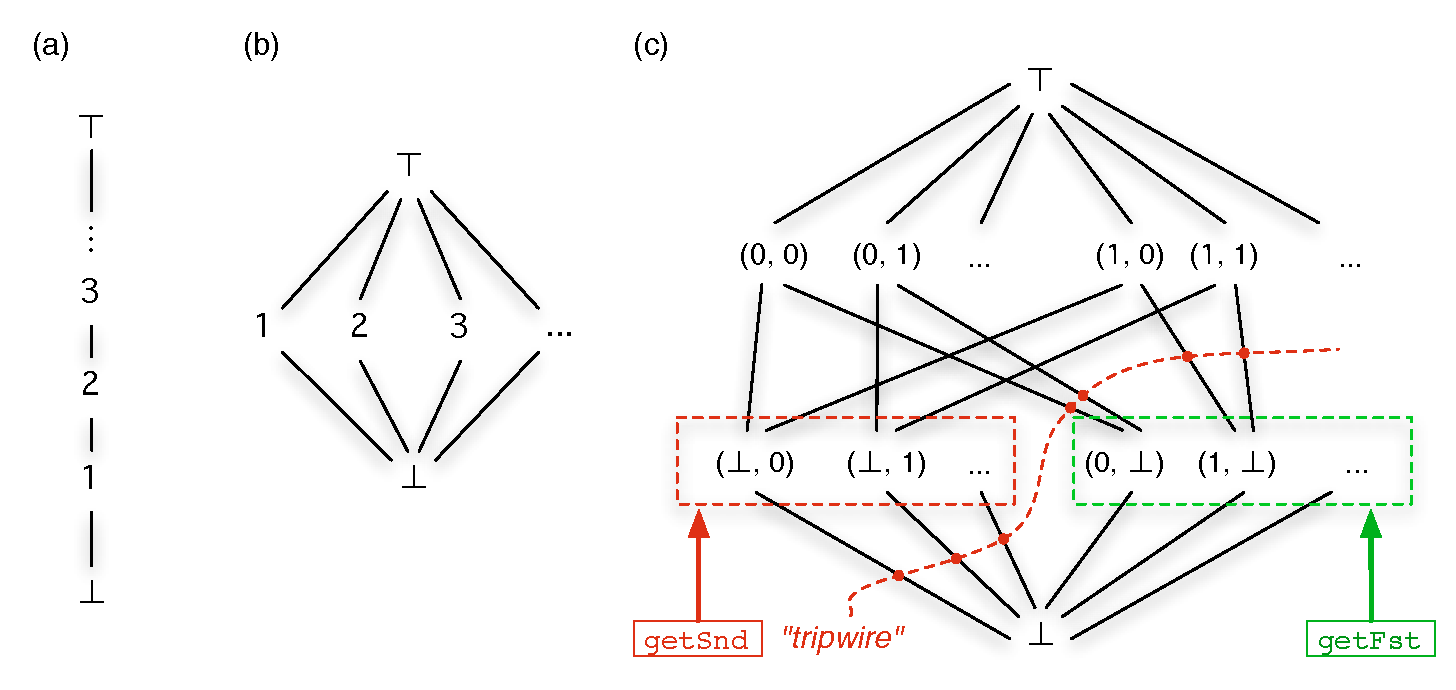
\includegraphics[width=5in]{chapter2/figures/lvars-example-lattices.pdf} 
  \caption{Example LVar lattices: (a) positive integers ordered by
    $\leq$; (b) IVar containing a positive integer; (c) pair of
    natural-number-valued IVars, annotated with example threshold sets
    that would correspond to a blocking read of the first or second
    element of the pair.  Any state transition crossing the
    ``tripwire'' for \termfont{getSnd} causes it to unblock and return
    a result.}
  \label{f:lvars-example-lattices}
\end{figure}

If $\mathit{lv}$'s lattice is the $\leq$ ordering on positive
integers, as shown in Figure~\ref{f:lvars-example-lattices}(a), then
$\mathit{lv}$'s state will always be $\max(3, 2) = 3$ by the time
$\GET~\mathit{lv}$ runs, since the least upper bound of two positive
integers $n_1$ and $n_2$ is $\max(n_1, n_2)$.  Therefore
\ref{e:lvar-example-1} will deterministically evaluate to $3$,
regardless of the order in which the two @put@ operations occurred.

On the other hand, if $\mathit{lv}$'s lattice is that shown in
Figure~\ref{f:lvars-example-lattices}(b), in which the least upper
bound of any two distinct positive integers is $\top$, then
\ref{e:lvar-example-1} will deterministically raise an exception,
indicating that conflicting writes to $\mathit{lv}$ have occurred.
This exception is analogous to the ``multiple @put@'' error raised
upon multiple writes to an IVar.  Unlike with a traditional IVar,
though, multiple writes of the \emph{same} value (say,
\putexp{\mathit{lv}}{3} and \putexp{\mathit{lv}}{3}) will \emph{not}
raise an exception, because the least upper bound of any positive
integer and itself is that integer---corresponding to the fact that
multiple writes of the same value do not allow any nondeterminism to
be observed.

\subsection{Threshold reads}

However, merely ensuring that writes to an LVar are monotonically
increasing is not enough to ensure that programs behave
deterministically.  Consider again the lattice of
Figure~\ref{f:lvars-example-lattices}(a) for $\mathit{lv}$, but
suppose we change \ref{e:lvar-example-1} to allow the @get@ operation
to be interleaved with the two @put@s:
\begin{equation}
\begin{split}
& \LETPAR ~\_ = \putexp{\mathit{lv}}{3} \\
&  \letparspace ~\_ = \putexp{\mathit{lv}}{2} \\
&  \letparspace ~x = \GET~\mathit{lv} \\
&  \letspace \IN~x
\end{split}
\label{e:lvar-example-2}
\end{equation}
Since the two @put@s and the @get@ can be scheduled in any order,
\ref{e:lvar-example-2} is nondeterministic: $x$ might be either $2$ or
$3$, depending on the order in which the LVar effects occur.
Therefore, to maintain determinism, LVars put an extra restriction on
the @get@ operation.  Rather than allowing @get@ to observe the exact
value of the LVar, it can only observe that the LVar has reached one
of a specified set of \emph{lower bound} states.  This set of lower
bounds, which we provide as an extra argument to @get@, is called a
\emph{threshold set} because the values in it form a ``threshold''
that the state of the LVar must cross before the call to @get@ is
allowed to unblock and return.  When the threshold has been reached,
@get@ unblocks and returns \emph{not} the exact value of the LVar, but
instead, the (unique) element of the threshold set that has been
reached or surpassed.

We can make \ref{e:lvar-example-2} behave deterministically by passing
a threshold set argument to @get@:
\begin{equation}
\begin{split}
& \LETPAR ~\_ = \putexp{\mathit{lv}}{3} \\
&  \letparspace ~\_ = \putexp{\mathit{lv}}{2} \\
&  \letparspace ~x = \getexp{\mathit{lv}}{\setof{3}} \\
&  \letspace \IN~x
\end{split}
\label{e:lvar-example-3}
\end{equation}
For instance, suppose we choose the singleton set $\setof{3}$ as the
threshold set.  Since $\mathit{lv}$'s value can only increase with
time, we know that once it is at least $3$, it will remain at or above
$3$ forever; therefore the program will deterministically evaluate to
$3$.  Had we chosen $\setof{2}$ as the threshold set, the program
would deterministically evaluate to $2$; had we chosen $\setof{4}$, it
would deterministically block forever.

As long as we only access LVars with @put@ and (thresholded) @get@, we
can arbitrarily share them between threads without introducing
nondeterminism. That is, the @put@ and @get@ operations in a given
program can happen in any order, without changing the value to which
the program evaluates.

\subsection{Incompatibility of threshold sets}

While the LVar interface just described is deterministic, it is only useful for
synchronization, not for communicating data: we must specify in advance the
single answer we expect to be returned from the call to @get@.  In general,
though, threshold sets do not have to be singleton sets.  For example, consider
an LVar $\mathit{lv}$ whose states form a lattice of \emph{pairs} of
natural-number-valued IVars; that is, $\mathit{lv}$ is a pair $(m, n)$, where
$m$ and $n$ both start as $\bot$ and may each be updated once with a non-$\bot$
value, which must be some natural number.
This lattice is shown in Figure~\ref{f:lvars-example-lattices}(c).

We can then define $\GETFST$ and
$\GETSND$ operations for reading from the first and second entries of
$\mathit{lv}$:
\begin{align*}
\getfstexp{p} & \defeq \getexp{p}{\stateset{(m, \bot) \setsep m \in
    \mathbb{N}}} \\
\getsndexp{p} & \defeq \getexp{p}{\stateset{(\bot, n) \setsep n \in
    \mathbb{N}}}
\end{align*}
This allows us to write programs like the following:
\begin{equation}
\begin{split}
& \LETPAR ~\_ = \putexp{\mathit{lv}}{(\bot, 4)} \\
&  \letparspace ~\_ = \putexp{\mathit{lv}}{(3, \bot)} \\
&  \letparspace ~x = \getsndexp{\mathit{lv}} \\
&  \letspace \IN~x
\end{split}
\label{e:lvar-example-4}
\end{equation}
In the call $\getsndexp{\mathit{lv}}$, the threshold set is
$\setof{(\bot, 0), (\bot, 1), \dots}$, an infinite set.  There is no
risk of nondeterminism because the elements of the threshold set are
\emph{pairwise incompatible} with respect to $\mathit{lv}$'s lattice:
informally, since the second entry of $\mathit{lv}$ can only be
written once, no more than one state from the set $\setof{(\bot, 0),
  (\bot, 1), \dots}$ can ever be reached.  (I formalize this
incompatibility requirement in
Section~\ref{subsection:lvars-communication-primitives}.)

In the case of \ref{e:lvar-example-4}, $\getsndexp{\mathit{lv}}$ may
unblock and return $(\bot, 4)$ any time after the second entry of
$\mathit{lv}$ has been written, regardless of whether the first entry
has been written yet.  It is therefore possible to use LVars to safely
read parts of an incomplete data structure---say, an object that is in
the process of being initialized by a constructor.

\subsection{The model versus reality}

The use of explicit threshold sets in the above LVars model should be
understood as a mathematical modeling technique, \emph{not} an
implementation approach or practical API.  The LVish library (which I
will discuss in Chapter~\ref{ch:lvish}) provides an unsafe @getLV@
operation to the authors of LVar data structure libraries, who can
then make operations like @getFst@ and @getSnd@ available as a safe
interface for application writers, implicitly baking in the particular
threshold sets that make sense for a given data structure without ever
explicitly constructing them.

To put it another way, operations on a data structure exposed as an
LVar must have the \emph{semantic effect} of a least upper bound for
writes or a threshold for reads, but none of this need be visible to
clients (or even written explicitly in the code).  Any data structure
API that provides such a semantics is guaranteed to provide
deterministic concurrent communication.
